%%% Hlavní soubor. Zde se definují základní parametry a odkazuje se na ostatní části. %%%

% Meta-data o práci (je nutno upravit)
\input metadata.tex

% Vygenerujeme metadata ve formátu XMP pro použití balíčkem pdfx
\input xmp.tex

%% Verze pro jednostranný tisk:
% Okraje: levý 40mm, pravý 25mm, horní a dolní 25mm
% (ale pozor, LaTeX si sám přidává 1in)
\documentclass[12pt,a4paper]{report}
\setlength\textwidth{145mm}
\setlength\textheight{247mm}
\setlength\oddsidemargin{15mm}
\setlength\evensidemargin{15mm}
\setlength\topmargin{0mm}
\setlength\headsep{0mm}
\setlength\headheight{0mm}
% \openright zařídí, aby následující text začínal na pravé straně knihy
\let\openright=\clearpage

%% Pokud tiskneme oboustranně:
% \documentclass[12pt,a4paper,twoside,openright]{report}
% \setlength\textwidth{145mm}
% \setlength\textheight{247mm}
% \setlength\oddsidemargin{14.2mm}
% \setlength\evensidemargin{0mm}
% \setlength\topmargin{0mm}
% \setlength\headsep{0mm}
% \setlength\headheight{0mm}
% \let\openright=\cleardoublepage

%% Pokud práci odevzdáváme pouze elektronicky, vypadají lépe symetrické okraje
% \documentclass[12pt,a4paper]{report}
% \setlength\textwidth{145mm}
% \setlength\textheight{247mm}
% \setlength\oddsidemargin{10mm}
% \setlength\evensidemargin{10mm}
% \setlength\topmargin{0mm}
% \setlength\headsep{0mm}
% \setlength\headheight{0mm}
% \let\openright=\clearpage

%% Vytváříme PDF/A-2u
\usepackage[a-2u]{pdfx}

%% Přepneme na českou sazbu a fonty Latin Modern
\usepackage[czech]{babel}
\usepackage{lmodern}

% Pokud nepouživáme LuaTeX, je potřeba ještě nastavit kódování znaků
\usepackage{iftex}
\ifpdftex
\usepackage[utf8]{inputenc}
\usepackage[T1]{fontenc}
\usepackage{textcomp}
\fi

%%% Další užitečné balíčky (jsou součástí běžných distribucí LaTeXu)
\usepackage{amsmath}        % rozšíření pro sazbu matematiky
\usepackage{amsfonts}       % matematické fonty
\usepackage{amsthm}         % sazba vět, definic apod.
\usepackage{bm}             % tučné symboly (příkaz \bm)
\usepackage{booktabs}       % lepší vodorovné linky v tabulkách
\usepackage{caption}        % umožní definovat vlastní popisky plovoucích objektů
\usepackage{csquotes}       % uvozovky závislé na jazyku
\usepackage{dcolumn}        % vylepšené zarovnání sloupců tabulek
\usepackage{floatrow}       % umožní definovat vlastní typy plovoucích objektů
\usepackage{graphicx}       % vkládání obrázků
\usepackage{icomma}         % inteligetní čárka v matematickém módu
\usepackage{indentfirst}    % zavede odsazení 1. odstavce kapitoly
\usepackage[nopatch=item]{microtype}  % mikrotypografická rozšíření
\usepackage{paralist}       % lepší enumerate a itemize
\usepackage[nottoc]{tocbibind} % zajistí přidání seznamu literatury,
                            % obrázků a tabulek do obsahu
\usepackage{xcolor}         % barevná sazba

% Balíček hyperref, kterým jdou vyrábět klikací odkazy v PDF,
% ale hlavně ho používáme k uložení metadat do PDF (včetně obsahu).
% Většinu nastavítek přednastaví balíček pdfx.
\hypersetup{unicode}
\hypersetup{breaklinks=true}

% Balíčky pro sazbu informatických prací
\usepackage{algpseudocode}  % součást balíčku algorithmicx
\usepackage[Algoritmus]{algorithm}
\usepackage{fancyvrb}       % vylepšené prostředí verbatim
\usepackage{listings}       % zvýrazňování syntaxe zdrojových textů

% Cleveref může zjednodušit odkazování, ale jeho užitečnost pro češtinu
% je minimalní, protože nezvládá skloňování.
% \usepackage{cleveref}

% Formátování bibliografie (odkazů na literaturu)
% Detailní nastavení můžete upravit v souboru macros.tex.
%
% POZOR: Zvyklosti různých oborů a kateder se liší. Konzultujte se svým
% vedoucím, jaký formát citací je pro vaši práci vhodný!
%
% Základní formát podle normy ISO 690 s číslovanými odkazy
\usepackage[natbib,style=iso-numeric,sorting=none]{biblatex}
% ISO 690 s alfanumerickými odkazy (zkratky jmen autorů)
%\usepackage[natbib,style=iso-alphabetic]{biblatex}
% ISO 690 s citacemi tvaru Autor (rok)
%\usepackage[natbib,style=iso-authoryear]{biblatex}
%
% V některých oborech je běžnější obyčejný formát s číslovanými odkazy
% (sorting=none říká, že se bibliografie má řadit podle pořadí citací):
%\usepackage[natbib,style=numeric,sorting=none]{biblatex}
% Číslované odkazy, navíc se [1,2,3,4,5] komprimuje na [1-5]
%\usepackage[natbib,style=numeric-comp,sorting=none]{biblatex}
% Obyčejný formát s alfanumerickými odkazy:
%\usepackage[natbib,style=alphabetic]{biblatex}

% Z tohoto souboru se načítají položky bibliografie
\addbibresource{literatura.bib}

% Definice různých užitečných maker (viz popis uvnitř souboru)
\input macros.tex

%%% Titulní strana a různé povinné informační strany
\begin{document}
%%% Titulní strana práce a další povinné informační strany

%%% Nápisy na přední straně desek
%%% Pokud je práce ve slovenštině, desky mají být česky.

% Desky obvykle nesázíme, ale pokud je chcete přidat, změnte \iffalse na \iftrue
\iffalse

\pagestyle{empty}
\hypersetup{pageanchor=false}
\begin{center}

\large
Univerzita Karlova

\medskip

Matematicko-fyzikální fakulta

\vfill

{\huge\bf\ThesisTypeTitle}

\vfill

{\huge\bf\ThesisTitle\par}

\vfill
\vfill

\hbox to \hsize{\YearSubmitted\hfil \ThesisAuthor}

\end{center}

\newpage\openright
\setcounter{page}{1}

\fi

%%% Titulní strana práce
%%% Pokud je práce ve slovenštině, tato strana zůstává česky.

\pagestyle{empty}
\hypersetup{pageanchor=false}

\begin{center}

\centerline{\mbox{\includegraphics[width=166mm]{img/logo-cs.pdf}}}

\vspace{-8mm}
\vfill

{\bf\Large\ThesisTypeTitle}

\vfill

{\LARGE\ThesisAuthor}

\vspace{15mm}

{\LARGE\bfseries\ThesisTitle\par}

\vfill

\Department

\vfill

{
\centerline{\vbox{\halign{\hbox to 0.45\hsize{\hfil #}&\hskip 0.5em\parbox[t]{0.45\hsize}{\raggedright #}\cr
Vedoucí \ThesisTypeGenitive{} práce:&\Supervisor \cr
\ifx\ThesisType\TypeRig\else
\noalign{\vspace{2mm}}
Studijní program:&\StudyProgramme \cr
\fi
}}}}

\vfill

Praha \YearSubmitted

\end{center}

\newpage

%%% Strana s čestným prohlášením k práci
%%% Pokud je práce ve slovenštině, tato strana zůstává česky.

\openright
\hypersetup{pageanchor=true}
\vglue 0pt plus 1fill

\noindent
Prohlašuji, že jsem tuto \ThesisTypeAccusative{} práci vypracoval(a) samostatně a výhradně
s~použitím citovaných pramenů, literatury a dalších odborných zdrojů.
Beru na~vědomí, že se na moji práci vztahují práva a povinnosti vyplývající
ze zákona č. 121/2000 Sb., autorského zákona v~platném znění, zejména skutečnost,
že Univerzita Karlova má právo na~uzavření licenční smlouvy o~užití této
práce jako školního díla podle §60 odst. 1 autorského zákona.

\vspace{10mm}

\hbox{\hbox to 0.5\hsize{%
V \hbox to 6em{\dotfill} dne \hbox to 6em{\dotfill}
\hss}\hbox to 0.5\hsize{\dotfill\quad}}
\smallskip
\hbox{\hbox to 0.5\hsize{}\hbox to 0.5\hsize{\hfil Podpis autora\hfil}}

\vspace{20mm}
\newpage

%%% Poděkování

\openright

\noindent
\Dedication

\newpage

%%% Povinná informační strana práce

\openright
{\InfoPageFont

\vtop to 0.5\vsize{
\setlength\parindent{0mm}
\setlength\parskip{5mm}

Název práce:
\ThesisTitle

Autor:
\ThesisAuthor

\DeptType:
\Department

Vedoucí \ThesisTypeGenitive{} práce:
\Supervisor, \SupervisorsDepartment

Abstrakt:
\Abstract

Klíčová slova:
{\def\sep{\unskip, }\ThesisKeywords}

\vfil
}

\vtop to 0.49\vsize{
\setlength\parindent{0mm}
\setlength\parskip{5mm}

Title:
\ThesisTitleEN

Author:
\ThesisAuthor

\DeptTypeEN:
\DepartmentEN

Supervisor:
\Supervisor, \SupervisorsDepartmentEN

Abstract:
\AbstractEN

Keywords:
{\def\sep{\unskip, }\ThesisKeywordsEN}

\vfil
}

}

\newpage

%%% Další stránky budeme číslovat
\pagestyle{plain}


%%% Strana s automaticky generovaným obsahem práce

\tableofcontents


%%% Použité zkratky v práci (opět nemusí být nutné uvádět)
%%% U matematických prací může být lepší přemístit seznam zkratek na začátek práce.
\chapter*{Used terms}
\addcontentsline{toc}{chapter}{Used Terms}


%%% Jednotlivé kapitoly práce jsou pro přehlednost uloženy v samostatných souborech
\chapter*{Úvod}
\addcontentsline{toc}{chapter}{Úvod}

Cílem této práce je prozkoumat několik moderních přístupů k vykreslování grafů, ať už softwaru nebo algoritmů.
Na základě těchto poznatků potom vytvořím vlastní software,
kde se pokusím vykreslovat velké grafy a to uživatelsky přívětivým způsobem přes webové rozhraní.

Konečným cílem mé práce je na tomto zobrazení postavit sociální síť, která bude pomocí grafu vizuálně reprezentovat aktuálně relevantní příspěvky.
Zároveň by tato síť měla uživatelům poskytnout vlastní filtry/vyhledávání, které bude taktéž zobrazovat výsledky coby graf.
%%% Fiktivní kapitola s ukázkami sazby

% \chapter{Související práce - Software}

% Softwaru vykreslujícím grafy je k dnešnímu dni mnoho a slouží k různým účelům.
% K porovnání s mou softwarové prací vyberu tři - každý s jiným zaměřením.

% Prvním bude Obsidian, který primárně slouží k managementu poznámek a grafový pohled
% na ně poskytuje jako zajímavou vlastnost navíc. Druhým je program Gephi, který se zaměřuje na studium a
% vykreslování velkých grafů a třetí bude knihovna pro vykreslování grafů na webu - Cytoscape.js.

% V rámci seznámení se s těmito systémy jsem se pokusil vykreslit jeden velký graf v každém z nich.
% Zajímalo mě, jak se chovají - a to jak kvalitativně, tak uživatelsky.
% Jako zdroj dat jsem použil dataset vzájemných citací publikací z oboru vysokoenergetické fyziky (https://snap.stanford.edu/data/cit-HepPh.html) \xxx{todo - správná citace},
% který má 34546 vrcholů a 421578 hran (níže označen jako CitHep).

\chapter{Related software}

There are plenty of programs and libraries for graph visualization with different purposes.
Just to name a few there are D3.js, Neo4j, Graphviz, Tulip, Wolfram Grapher, Pajek and many more.

In this chapter however I'm going to focus on just three software products - each with very different use-case and target userbase.

\begin{itemize}

\item The first one is \textbf{Obsidian} which is primarily a note-taking application
but provides a graph view of the notes as an interesting and easy to use feature. 

\item The second is \textbf{Gephi}, a software focused on in-depth analysis and visualization of large graphs.

\item And finally there's \textbf{Cytoscape.js}. A javascript library for graph visualization in the browser.

\end{itemize}

I chose these in particular because in later chapters I'm going to build a software that could be viewed as a hybrid of the three.

We will look into three aspects of these products:
\begin{itemize}
  \item Primary use-case and target userbase
  \item User experience
  \item Ability to visualize large graphs
\end{itemize}

As the source of data for testing the large-graph visualization capabilities I chose the dataset of citations between papers
in the field of high-energy physics \xxx{(CitHep) \cite{snap_cit_hep}} (Later refered to as the CitHep dataset).
It contains 34546 nodes, 421578 edges and temporal data.

This dataset is suitable for my purposes because:
\begin{itemize}
  \item It's large enough to test the limits of both the mentioned software and Afantázie
  \item It's a real-world dataset with temporal data which is going to play a role in visualizing the contents of Afantázie
\end{itemize}

\section{Obsidian}

% Obsidian byla přímá inspirace pro tento projekt. Umožňuje vytvářet,
% editovat a hlavně navzájem provázat poznámky coby markdown soubory v souborovém systému.

% Jeho grafový renderer je animovaný a simuluje v grafu několik sil
% - jednotlivé poznámky se přitahují, jsou-li spojené hranou (jinak řečeno na sebe odkazují),
% odpuzují se, pokud jsou moc blízko a všechny vrcholy jsou ovlivněné gravitací, která celý graf vycentruje.
% (Toto je velmi běžný přístup k vykreslování grafů, známý jako \textit{force-directed layout} \xxx{více v kapitole todo}).
% Uživatel má k
% dispozici posuvníky, kterými může tyto síly a některé další parametry upravovat a tím v reálném
% čas plynule měnit, jak graf vypadá.

% Obsidian je výborný nástroj pro management poznámek, ale jeho grafový pohled je spíše vedlejší funkcí.
% Tomu odpovídá i míra jeho konfigurovatelnosti - uživatel sice má možnost měnit barvy vrcholů, podle různých filtrů,
% ale výsledné rozložení grafu může ovlivnit pouze posuvníky \textit{center force, repel force, link force a link distance}.
% Tyto parametry jsou dostačující pro malé grafy, avšak větší grafy neposkytují moc dobré shlukování.

Obsidian was a direct inspiration for Afantázie. It allows users to create, edit and most importantly interlink markdown file notes in the file system.
One Obsidian project is just a system directory called a Vault. It is a set of markdown notes, user settings, plugins and other files.
The interlinked notes in a Vault form a directed graph which can be visualized with just a click of a button.
The graph is animated and has the ability to replay the history of the Vault from the very first note to the current state.

It's clear from this description that Obsidian is aimed at general audience of note-takers 
with maybe a slight bias towards graph/data visualization enthisuiasts.
It's available for all the major operating systems and has a large community of users and plethera of extensions available through the community plugins.

\subsection{Obsidian graph view limitations}

The graph visualization in obsidian (from here on called graph view) is based on a force-directed layout algorithm \xxx{(more in chapter TBD)}.
It is easy to use and provides an appealing visual representation of the notes. It is also customizable to some extent.
Colors of the nodes can be set based on different filters such as path, tags or text-search.
Users can also adjust four sliders - central force, repel force, link force and link distance.
In figure \ref{obr:obsidian_common} you can see a typical Obsidian graph view depicting a Vault of one of my personal projects.

The customization is sufficient for small graphs but for larger graphs the program spends some time indexing the notes.
(Though, this is a one-time operation and the index is then saved in the Vault).

In figure \ref{obr:obsidian_3000} you can see a part of the CitHep dataset with only the first 3000 nodes.
It took my machine over 10 minutes to index this graph and I was unable to visualize the whole dataset without the program crashing or taking too long to index.
Once indexed however the application ran smoothly and the graph view produced was visually appealing.

However, Obsidian is not very good at clustering nodes with high degree of connectivity.
It also has no support for automatic colouring of the nodes based on clusters, modularity \xxx{(check this <-)} or other data indicators.
Color has to be user defined which is why the graph in figure \ref{obr:obsidian_3000} is all gray.


\xxx{TODO - proportions of the image(s)}
\begin{figure}[p]\centering
  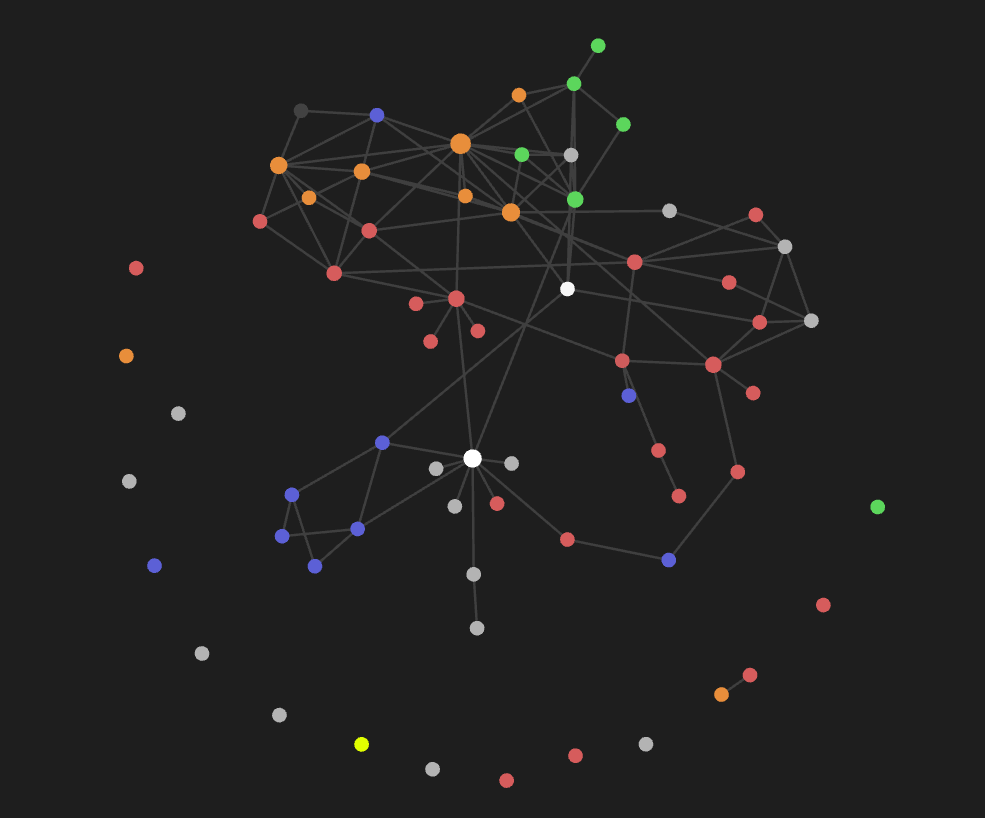
\includegraphics[width=140mm, height=140mm]{img/obsidian_common_notes.png}
  \caption{A common graph view of a small Vault in Obsidian}
  \label{obr:obsidian_common}
\end{figure}

% \subsection{Limity}
% Vzhledem k zamýšlenému účelu nemá Obsidian dobrou podporu pro velké grafy.
% Jde to, avšak pouze s dlouhým časem indexování \xxx{(todo - vysvětlovat nebo ne?)} a je těžkopádné editovat jak výsledné rozložení, tak vzhled grafu.

% Na obrázku \ref{obr:obsidian_3000} je vyobrazena část datasetu CitHep, která obsahuje pouze prvních 3000 vrcholů.
% Nepovedlo se mi zobrazit celý dataset, aniž by aplikace spadla nebo trvalo indexování příliš dlouho.
% Indexování tohoto grafu zabralo přes 15 minut.


\begin{figure}[p]\centering
  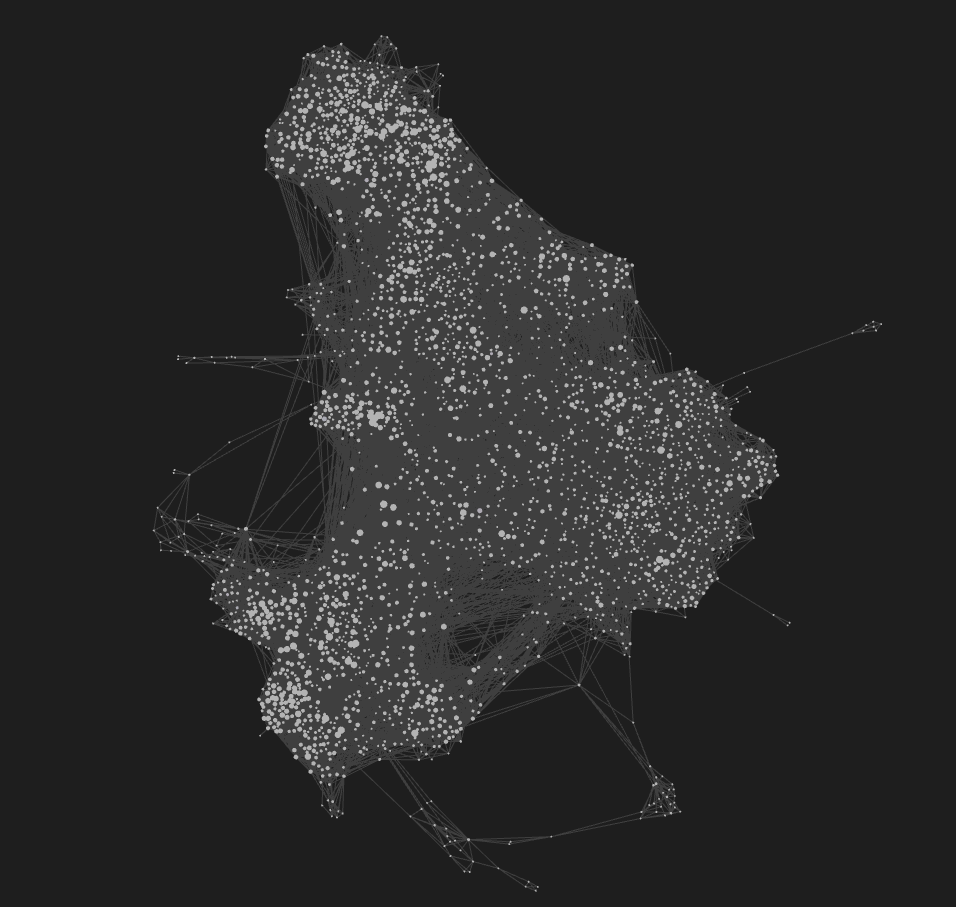
\includegraphics[width=140mm, height=140mm]{img/Obsidian_3000}
  \caption{The first 3000 nodes of the CitHep dataset visualized in Obsidian}
  \label{obr:obsidian_3000}
\end{figure}

\section{Gephi}

% Gephi je software zaměřující se jak na vizualizaci tak na kvantitativní analýzu velkých grafů. Poskytuje množinu \textit{Layout algoritmů} \xxx{(viz kapitola TBD)}, pomocí 
% kterých lze inkrementálně upravovat rozložení a vzhled grafu. Používání tohoto softwaru vyžaduje jistou míru jak technických znalosti grafů a layout algoritmů
% tak ovládání programu jako takového.

% Výsledkem práce v Gephi je vyexportovaný obrázek. Jeho podobu lze velmi podrobně upravovat -
% mimo jiné v něm lze měnit barvy, velikosti vrcholů, tloušťky a zakřivení hran a to vše je možné nastavovat automaticky pomocí různých vlastností dat.

% Na obrázku \ref{obr:gephi_cithep} jsem vyobrazil kompletní dataset CitHep. Jde na něm vidět mnohem více datových indikátorů než v případě Obsidianu.

% Konkrétně:
% \begin{itemize}
%   \item Barva vrcholů značí komunitu, do které vrchol patří.
%   \item Velikost vrcholů značí počet citací, které na asociovanou studii odkazují
%   \item Layout má výraznější členění a jdou na něm lépe vidět jednotlivé komunity
% \end{itemize}

% Zobrazování grafů pomocí Gephi je relativně časově náročné, na rozdíl od Obsidianu, kde funguje implicitně a uživatelsky přívětivě.
% To však souvisí s jinými zaměřeními obou systémů.

Much more specialized than Obsidian, Gephi is an open source software focused on visualization and quantitative analysis of large graphs.
It provides tens and with plugins hundreds \xxx{(cit. needed)} algorithms for graph layout and quantitative analysis of various data.

Gephi can compute quantitative characteristics of the data and graphs such as modularity, clustering coefficient, degree distribution and many more.
It can not just vizualize the working data but it can export rather visually appealing images of the graph.

In figure \ref{obr:gephi_cithep_3k} you can see, again, the first 3000 nodes of the CitHep dataset visualized in Gephi.
Compared with Obsidian the Gephi redner provides more visually identifiable characteristics of the data:
\begin{itemize}
  \item The layout is more structured and communities are more visible
  \item Colors of the nodes represent their associated modularity class
  \item Size of the nodes represents the number of citations the associated paper has (or in-degree)
\end{itemize}


% \subsection{Limity}

% Gephi je jeden z nejlepších nástrojů, po kterém lze sáhnout při potřebě vizualizovat nebo analyzovat velké grafy a lze ji
% použít k vyobrazení takřka libovolného množství vrcholů a hran (v rámci limit hardwaru).

\begin{figure}[p]\centering
  \includegraphics[width=140mm, height=140mm]{img/gephi_first_3000.png}
  \caption{The first 3000 nodes of the CitHep dataset visualized in Gephi}
  \label{obr:gephi_cithep_3k}
\end{figure}


\begin{figure}[p]\centering
  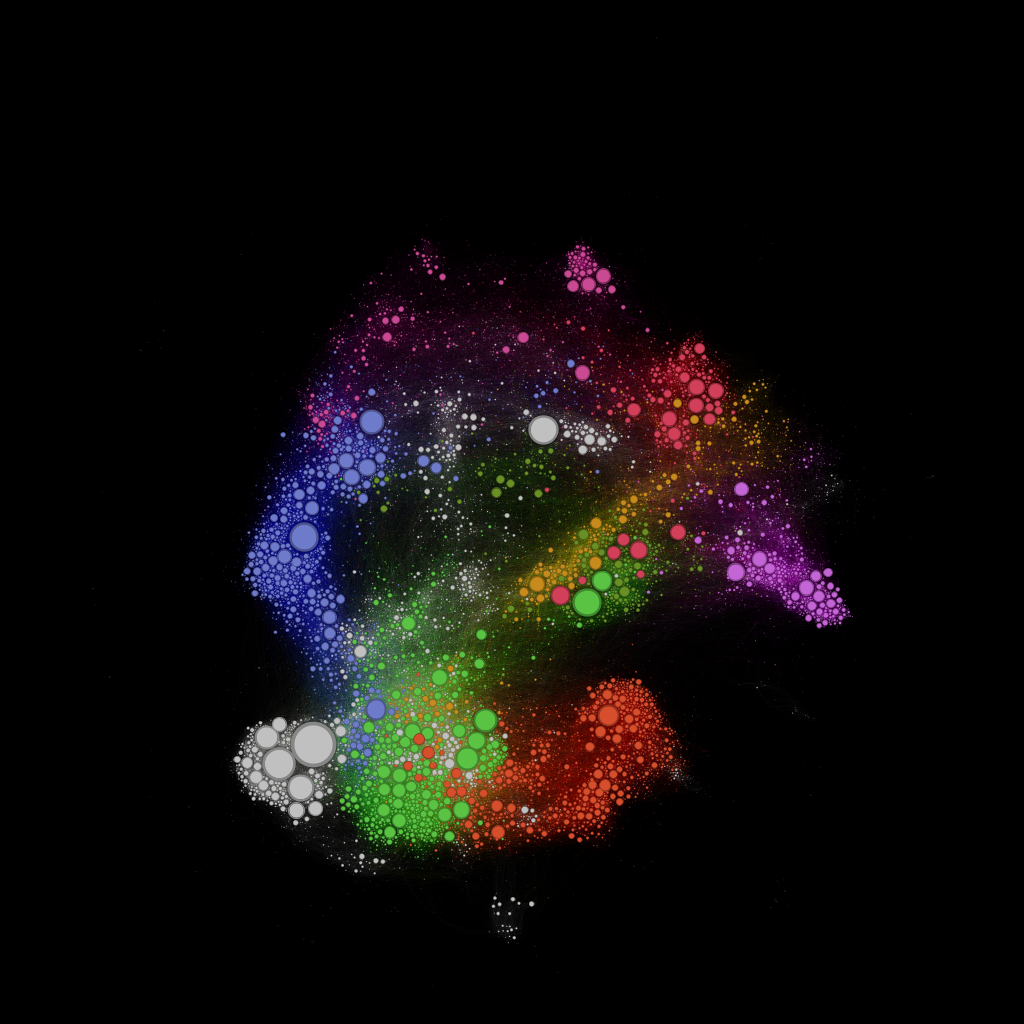
\includegraphics[width=140mm, height=140mm]{img/gephi_cithep_35k.png}
  \caption{The entire CitHep dataset visualized in Gephi (34546 nodes)}
  \label{obr:gephi_cithep}
\end{figure}

% Při takto velkém datasetu se aplikace znatelně sekala a práce v ní nebyla nejpříjemnější. Výsledky však mluví za sebe.

\section{Cytoscape.js}
Cytoscape.js je javascriptová knihovna, která umí renderovat grafy v prohlížeči pomocí canvasu. 
\xxx{TODO - Vyzkoušet}

\section{Afantázie}

Afantázie je název softwarového díla, které je výsledkem této práce. Jde o webovou stránku, na které moje poznatky související práce a grafových algoritmů aplikuji.
V porovnání se zmíněným softwarem bude Afantázie jistým kompromisem všech tří:

\begin{itemize}
  \item Stejně jako Obsidian bude graf na Afantázii uživatelsky přívětivý a uživatel bude moct přispět k datům, která jej tvoří
  \item Zaměřím se na metody, jak na stránce vykreslit velké množství vrcholů a tím se přiblížit schopnostem Gephi
  \item Podobně jako při použití Cytoscape bude graf přístupný z webového rozhraní
\end{itemize}
\chapter{Související práce - Algoritmy}

\section{Fruchterman-Reingold}

\section{OpenOrd}

\section{ForceAtlas}

\chapter{Webová stránka - prototyp}

\section{Účel}

\section{Technologie a architektura}

\section{Nasazení}
\chapter{Implementace webového vykreslování velkých grafů}

\section{Přehled implementace}

\section{Použité grafové algoritmy}

\section{Výsledky}

\chapter*{Závěr}
\addcontentsline{toc}{chapter}{Závěr}


%%% Seznam použité literatury
%%% Seznam použité literatury (bibliografie)
%%%
%%% Pro vytváření bibliografie používáme biblatex. Ten zpracovává
%%% citace v textu (např. makro \cite{...}) a vyhledává k nim literaturu
%%% v souboru literatura.bib.
%%%
%%% Podívejte se na nastavení biblatexu v souboru thesis.tex.

%%% Vytvoření seznamu literatury. Pozor, pokud jste necitovali ani jednu
%%% položku, seznam se automaticky vynechá.

% Dovolíme položkám trochu vyčuhovat přes pravý okraj.
\def\bibfont{\hfuzz=2pt}

\printbibliography[heading=bibintoc,title=Literatura]

%%% Kdybyste chtěli bibliografii vytvářet ručně (bez biblatexu), lze to udělat
%%% následovně. V takovém případě se řiďte normou ISO 690 a zvyklostmi v oboru.

% \begin{thebibliography}{99}
%
% \bibitem{lamport94}
%   {\sc Lamport,} Leslie.
%   \emph{\LaTeX: A Document Preparation System}.
%   2. vydání.
%   Massachusetts: Addison Wesley, 1994.
%   ISBN 0-201-52983-1.
%
% \end{thebibliography}


%%% Obrázky v práci
%%% (pokud jich je malé množství, obvykle není třeba seznam uvádět)
\listoffigures

%%% Tabulky v práci (opět nemusí být nutné uvádět)
%%% U matematických prací může být lepší přemístit seznam tabulek na začátek práce.
\listoftables


%%% Součástí doktorských prací musí být seznam vlastních publikací
\ifx\ThesisType\TypePhD
\chapwithtoc{Seznam publikací}
\fi

%%% Přílohy k práci, existují-li. Každá příloha musí být alespoň jednou
%%% odkazována z vlastního textu práce. Přílohy se číslují.
%%%
%%% Do tištěné verze se spíše hodí přílohy, které lze číst a prohlížet (dodatečné
%%% tabulky a grafy, různé textové doplňky, ukázky výstupů z počítačových programů,
%%% apod.). Do elektronické verze se hodí přílohy, které budou spíše používány
%%% v elektronické podobě než čteny (zdrojové kódy programů, datové soubory,
%%% interaktivní grafy apod.). Elektronické přílohy se nahrávají do SISu.
%%% Povolené formáty souborů specifikuje opatření rektora č. 72/2017.
%%% Výjimky schvaluje fakultní koordinátor pro zavěrečné práce.
\appendix
\chapter{Přílohy}

\section{První příloha}

\end{document}
